\documentclass[tikz,border=5mm]{standalone}
\usepackage[T1]{fontenc}
\usepackage{fontspec}
\setmainfont{Fira Sans}[
  BoldFont=Fira Sans Bold,
  ItalicFont=Fira Sans Italic,
]
\usetikzlibrary{positioning, arrows.meta, shadows.blur, calc}

\definecolor{mTeal}{HTML}{2B7A78}
\definecolor{mBrown}{HTML}{C9956B}
\definecolor{mRed}{HTML}{CC4444}
\definecolor{mGray}{HTML}{888888}
\definecolor{mBg}{HTML}{FAFAFA}

\begin{document}
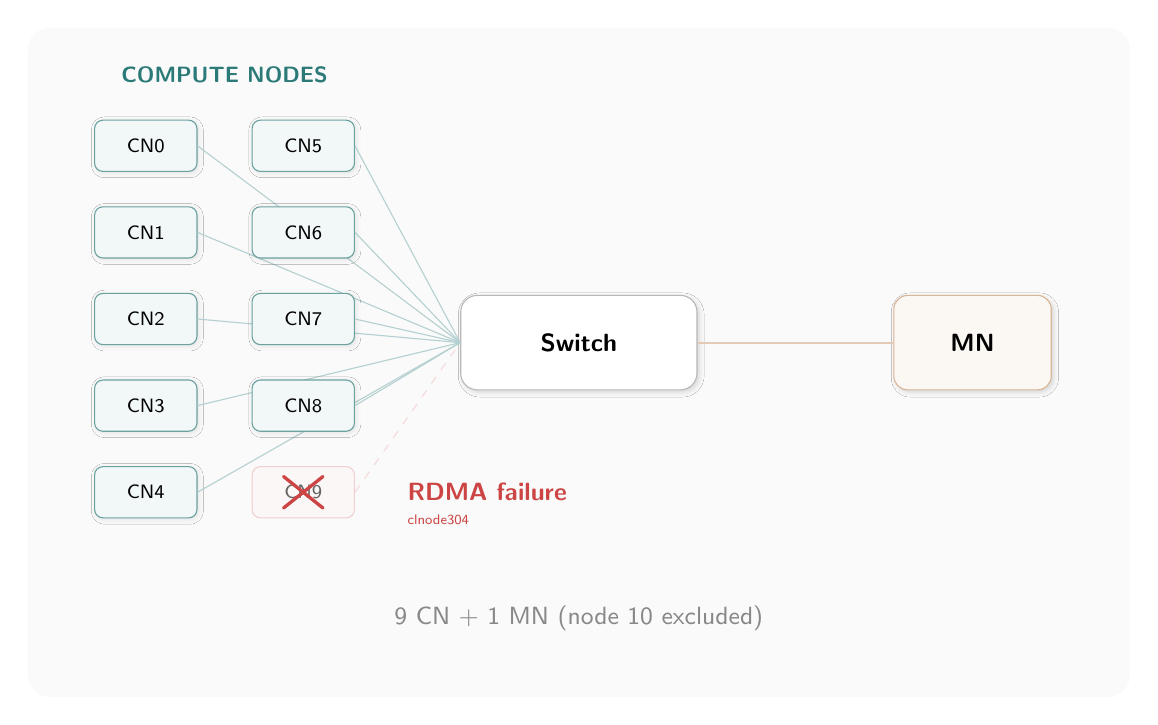
\begin{tikzpicture}[
  every node/.style={font=\sffamily},
  cn/.style={draw=mTeal!70, fill=mTeal!6, rounded corners=3pt,
             minimum width=1.3cm, minimum height=0.65cm, font=\sffamily\scriptsize,
             blur shadow={shadow blur steps=4, shadow xshift=0.2mm,
             shadow yshift=-0.2mm, shadow opacity=10}},
  dead/.style={draw=mRed!40, fill=mRed!5, rounded corners=3pt,
               minimum width=1.3cm, minimum height=0.65cm, font=\sffamily\scriptsize,
               opacity=0.6},
  sw/.style={draw=mGray!60, fill=white, rounded corners=6pt,
             minimum width=3cm, minimum height=1.2cm, font=\sffamily\small\bfseries,
             blur shadow={shadow blur steps=6, shadow xshift=0.3mm,
             shadow yshift=-0.3mm, shadow opacity=15}},
  mn/.style={draw=mBrown!70, fill=mBrown!8, rounded corners=5pt,
             minimum width=2cm, minimum height=1.2cm, font=\sffamily\small\bfseries,
             blur shadow={shadow blur steps=6, shadow xshift=0.3mm,
             shadow yshift=-0.3mm, shadow opacity=15}},
]
  \fill[mBg, rounded corners=8pt] (-7,-4.5) rectangle (7,4);
  \node[mTeal, font=\sffamily\footnotesize\bfseries] at (-4.5,3.4) {COMPUTE NODES};
  \node[sw] (switch) at (0,0) {Switch};
  \node[mn] (mn) at (5,0) {MN};
  \draw[mBrown!50, thick] (switch.east) -- (mn.west);

  \foreach \i [evaluate=\i as \y using {2.5-\i*1.1}] in {0,...,4} {
    \node[cn] (cn\i) at (-5.5, \y) {CN\i};
    \draw[mTeal!35, thin] (cn\i.east) -- (switch.west);
  }
  \foreach \i [evaluate=\i as \j using {int(\i+5)},
               evaluate=\i as \y using {2.5-\i*1.1}] in {0,...,3} {
    \node[cn] (cn\j) at (-3.5, \y) {CN\j};
    \draw[mTeal!35, thin] (cn\j.east) -- (switch.west);
  }

  % Broken node
  \node[dead] (cn9) at (-3.5, 2.5-4*1.1) {CN9};
  \draw[mRed!20, dashed, thin] (cn9.east) -- (switch.west);

  % X mark
  \draw[mRed, very thick, line cap=round] ($(cn9.center)+(-0.25,0.2)$) -- ($(cn9.center)+(0.25,-0.2)$);
  \draw[mRed, very thick, line cap=round] ($(cn9.center)+(-0.25,-0.2)$) -- ($(cn9.center)+(0.25,0.2)$);

  % Failure label
  \node[mRed, font=\sffamily\small\bfseries, anchor=west] at (-2.3, 2.5-4*1.1) {RDMA failure};
  \node[mRed, font=\sffamily\tiny, anchor=west] at (-2.3, 2.5-4*1.1-0.35) {clnode304};

  % Status
  \node[mGray, font=\sffamily\small] at (0,-3.5) {9 CN + 1 MN (node 10 excluded)};
\end{tikzpicture}
\end{document}
